\section{Reservoirdrücke}
\label{sec:reservoirs}


\begin{figure}[H]
    \centering
    \begin{subfigure}[H]{0.4\textwidth}
        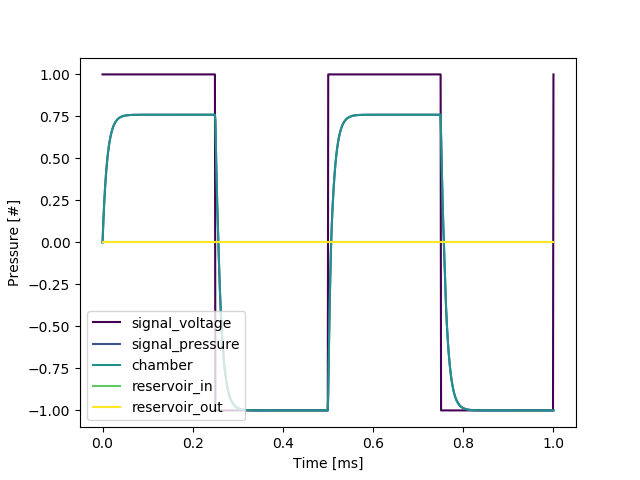
\includegraphics[width=\textwidth, valign=t]{plots/backpressure/backpressure_free.png}
        \caption{•}
    \end{subfigure}
    \begin{subfigure}[H]{0.4\textwidth}
        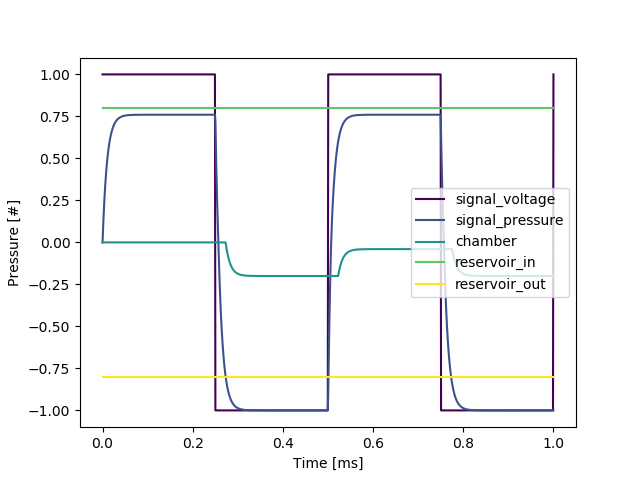
\includegraphics[width=\textwidth, valign=t]{plots/backpressure/backpressure_example.png}
        \caption{•}
    \end{subfigure}
    \caption{•}
\end{figure}

\begin{figure}[H]
    \centering
    \begin{subfigure}[H]{0.4\textwidth}
        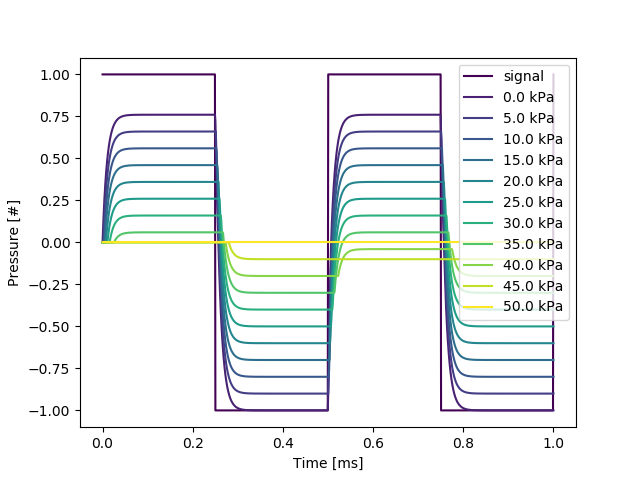
\includegraphics[width=\textwidth, valign=t]{plots/backpressure/backpressure_at_pr_in_and_pr_out.png}
        \caption{•}
    \end{subfigure}
    \begin{subfigure}[H]{0.4\textwidth}
        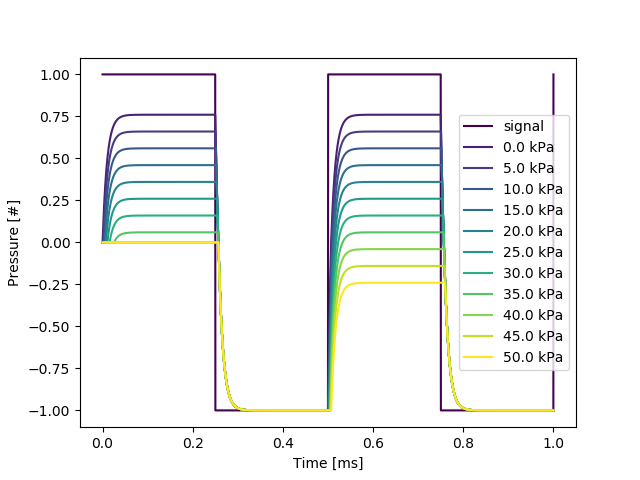
\includegraphics[width=\textwidth, valign=t]{plots/backpressure/backpressure_at_pr_in.png}
        \caption{•}
    \end{subfigure}
    \caption{•}
\end{figure}



\begin{figure}[H]
	\centering
	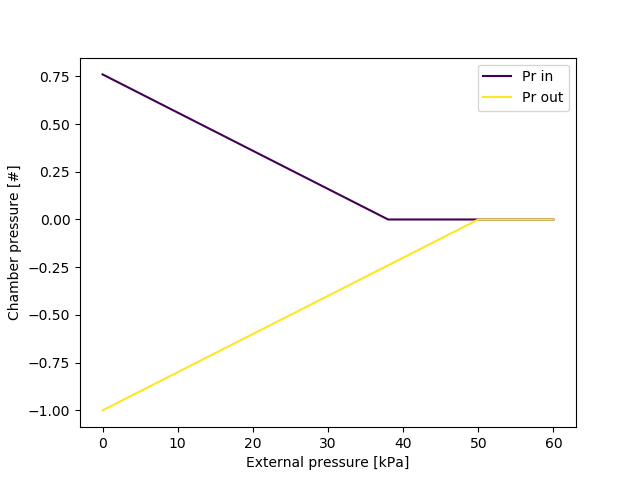
\includegraphics[width=0.7\textwidth]{plots/backpressure/backpressure_result.png}
	\caption{•}
\end{figure}